% This LaTeX was auto-generated from MATLAB code.
% To make changes, update the MATLAB code and export to LaTeX again.

\documentclass{article}

\usepackage[utf8]{inputenc}
\usepackage[T1]{fontenc}
\usepackage{lmodern}
\usepackage{graphicx}
\usepackage{color}
\usepackage{listings}
\usepackage{hyperref}
\usepackage{amsmath}
\usepackage{amsfonts}
\usepackage{epstopdf}
\usepackage{matlab}

\sloppy
\epstopdfsetup{outdir=./}
\graphicspath{ {./HW5_GrantRoberts_images/} }

\begin{document}

\matlabheading{\textit{Introduction}}

\begin{par}
\begin{flushleft}
In this MATLAB exercise we will investigate the phase of images acquired in a phantom and in vivo in respect to the echo time in a spoiled gradient echo sequence (aka SPGR aka FLASH). We will generate frequency maps and images that separate water and fat based on Dixon reconstruction techniques. The lecture slides on this topic should provide a solid basis for the analysis at hand. In addition, a write-up from Dr. John Pauly at Stanford University is provided.
\end{flushleft}
\end{par}

\begin{par}
\begin{flushleft}
\textbf{Please label all images properly: provide colorbars and a title. Also provide labels for x and y when you see it necessary. Make sure that the images are properly displayed in terms of their aspect ratio (hint: use truesize with imshow or axis image)}
\end{flushleft}
\end{par}

\vspace{1em}

\matlabheading{\textit{Problem 1 -- Phantom Data}}

\begin{par}
\begin{flushleft}
Read the phantom data set into Matlab. In this experiment, I placed 1 vial of fat on top of 2 vials of water. Those are single slice data that were acquired with a gradient echo sequence on a Siemens Sonata scanner. The TR was kept constant at 40 ms while the echo time TE was shifted from 4.0 ms (Series 01) to 6.0 ms (Series 02) and 8.0 ms (Series 03) corresponding to in and out of phase images or water and fat.
\end{flushleft}
\end{par}

\begin{par}
\begin{flushleft}
Note the difference in raw data format from the GE datasets that were provided in Homework \#2. For each Series, there is a data file (meas.out) and a text file (meas.asc). The text file contains details on the scan parameters (e.g. field of view, bandwidth, etc).
\end{flushleft}
\end{par}


\matlabheading{1a)}

\begin{par}
\begin{flushleft}
\textbf{Find the parameters for field of view and slice thickness in in the scan parameter file for Series 1 and report the values} (sSliceArray.asSlice[0].dThickness, sSliceArray.asSlice[0].dPhaseFOV, sSliceArray.asSlice[0].dReadoutFOV = 300 – all stored in mm). 
\end{flushleft}
\end{par}

\begin{par}
\begin{flushleft}
Tip: If you \textbf{change the extension of meas.asc to meas.txt}, your computer will associate the appropriate text editor with opening this file.
\end{flushleft}
\end{par}

\begin{matlabcode}
%%% Setup
close all

cd('../..')
% hw5dir = 'C:\Users\groberts\Documents\Fall 2018 Classwork\MP710\Homework\MP710_HW5_Files';
hw5dir = 'C:\Users\robertsgr\Documents\MP710\Homework\MP710_HW5_Files';
cd(hw5dir);                         % Start at home
addpath(genpath('.'))               % Add all subfolders to path

%%% Find parameters
cd('Data_Phantom')

% Convert all .asc files to .txt
DIR = dir('./*/*.asc');
for ii=1:length(DIR)
    filename = DIR(ii).name;
    cd(DIR(ii).folder)
    [pathstr, name, ext] = fileparts([DIR(ii).folder '\' filename]);
    copyfile(filename, fullfile(pathstr, [name, '.txt']));
end

%Read text file
cd('../01')
fileID = fopen('meas.asc');
Info = strtrim(textscan(fileID,'%s %s','Delimiter','='));
fclose(fileID);  

%Find specific values in text file
% This uses "lookup", a function defined at the end of this script.
% Lookup finds the value associated with a field.
field = Info{1}; value = Info{2};  
dZ = lookup(field,value,'sSliceArray.asSlice[0].dThickness',1);
FOVx = lookup(field,value,'sSliceArray.asSlice[0].dReadoutFOV',1);
FOVy = lookup(field,value,'sSliceArray.asSlice[0].dPhaseFOV',1);
TE = [4 6 8]; %ms

formatSpec = 'FOVx = %d mm, FOVy = %d mm, Slice thickness = %d mm';
sprintf(formatSpec,FOVx,FOVy,dZ)
\end{matlabcode}
\begin{matlaboutput}
ans = 'FOVx = 300 mm, FOVy = 300 mm, Slice thickness = 10 mm'
\end{matlaboutput}

\matlabheading{1b)}

\begin{par}
\begin{flushleft}
\textbf{Read the raw k-space data into Matlab }and generate the corresponding images for each echo time. I prepared a routine read\_raw\_form\_n4.m to read the data and I also posted a mini script script\_read\_phantom.m to show you how to use it. \textbf{Provide the resulting images (magnitude and phase) for all 3 echoes.}
\end{flushleft}
\end{par}

\begin{matlabcode}
%Read phantom data
script_read_phantom
\end{matlabcode}
\begin{matlaboutput}
Read image volume: 256 x 256 x 3
\end{matlaboutput}
\begin{matlabcode}
im = im_vol; clear im_vol;
mag = abs(im);
phase = angle(im);

% % Magnitude
figure; subplot(3,1,1); imshow(mag(:,:,1),[]);  title('Magnitude (Out of Phase -180)'); colorbar; map1 = colorbar; title(map1,'[a.u.]');
subplot(3,1,2); imshow(mag(:,:,2),[]);  title('Magnitude (In Phase)'); colorbar; map2 = colorbar; title(map2,'[a.u.]');
subplot(3,1,3); imshow(mag(:,:,3),[]);  title('Magnitude (Out of Phase +180'); colorbar; map3 = colorbar; title(map3,'[a.u.]');
\end{matlabcode}
\begin{center}
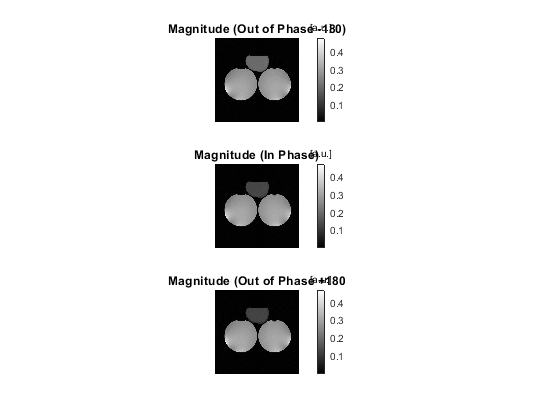
\includegraphics[width=\maxwidth{56.196688409433015em}]{figure_0}
\end{center}
\begin{matlabcode}

% Phase
figure; subplot(3,1,1); imshow(phase(:,:,1),[]);  title('Phase (Out of Phase -180)'); colorbar; map1 = colorbar; title(map1,'[rad]');
subplot(3,1,2); imshow(phase(:,:,2),[]);  title('Phase (In Phase)'); colorbar; map2 = colorbar; title(map2,'[rad]');
subplot(3,1,3); imshow(phase(:,:,3),[]);  title('Phase (Out of Phase +180 '); colorbar; map3 = colorbar; title(map3,'[rad]');
\end{matlabcode}
\begin{center}
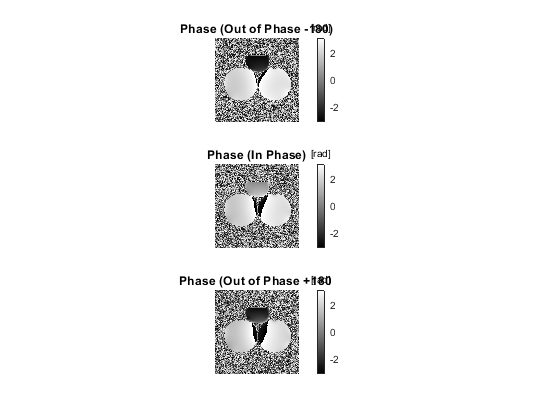
\includegraphics[width=\maxwidth{56.196688409433015em}]{figure_1}
\end{center}

\matlabheading{1c)}

\begin{par}
\begin{flushleft}
\textbf{Draw regions of interest in each of the 3 vials and create plots of signal vs echo time and phase vs echo time}. Remember that phase wraps may occur and try to compensate for those. \textbf{Describe the results}.
\end{flushleft}
\end{par}

\begin{matlabcode}
%Phase Unwrap
\end{matlabcode}

\vspace{1em}

\begin{par}
\begin{flushleft}
\underline{Vial \#1 - Far Left}
\end{flushleft}
\end{par}

\begin{matlabcode}
figure; subplot(3,1,1);
imshow(mag(:,:,1),[]);
ROI1 = drawrectangle('Color','g','Label','ROI1');
title('Vial #1 (Far Left)');
i1 = floor(ROI1.Position);          % Position of the ROI [xmin, ymin, width, height]
                                    % xmin and ymin = upper left corner of ROI
rows1 = i1(2):(i1(2)+i1(4));
cols1 = i1(1):(i1(1)+i1(3));

% The signal will be averaged over the ROI for magnitude and phase images.
S1mag = zeros(1,3);
for ii=1:3
    S1mag(ii) = mean2(mag(rows1,cols1,ii)); % Get mean for each time frame
end
S1phase = zeros(1,3);
for ii=1:3
    S1phase(ii) = mean2(phase(rows1,cols1,ii)); % Get mean for each time frame
end
\end{matlabcode}

\begin{par}
\begin{flushleft}
\underline{Vial \#2 - Upper-Middle }
\end{flushleft}
\end{par}

\begin{matlabcode}
subplot(3,1,2);
imshow(mag(:,:,1),[]);
ROI2 = drawrectangle('Color','g','Label','ROI2');
title('Vial #2 (Upper Middle)');
i2 = floor(ROI2.Position);          % Position of the ROI [xmin, ymin, width, height]
                                    % xmin and ymin = upper left corner of ROI
rows2 = i2(2):(i2(2)+i2(4));
cols2 = i2(1):(i2(1)+i2(3));

% The signal will be averaged over the ROI for magnitude and phase images.
S2mag = zeros(1,3);
for ii=1:3
    S2mag(ii) = mean2(mag(rows2,cols2,ii)); % Get mean for each time frame
end
S2phase = zeros(1,3);
for ii=1:3
    S2phase(ii) = mean2(phase(rows2,cols2,ii)); % Get mean for each time frame
end
\end{matlabcode}

\begin{par}
\begin{flushleft}
\underline{Vial \#3 - Far Right}
\end{flushleft}
\end{par}

\begin{matlabcode}
subplot(3,1,3);
imshow(mag(:,:,1),[]);
ROI3 = drawrectangle('Color','g','Label','ROI3');
title('Vial #3 (Far Right)');
i3 = floor(ROI3.Position);          % Position of the ROI [xmin, ymin, width, height]
                                    % xmin and ymin = upper left corner of ROI
rows3 = i3(2):(i3(2)+i3(4));
cols3 = i3(1):(i3(1)+i3(3));

% The signal will be averaged over the ROI for magnitude and phase images.
S3mag = zeros(1,3);
for ii=1:3
    S3mag(ii) = mean2(mag(rows3,cols3,ii)); % Get mean for each time frame
end
S3phase = zeros(1,3);
for ii=1:3
    S3phase(ii) = mean2(phase(rows3,cols3,ii)); % Get mean for each time frame
end

\end{matlabcode}

\begin{par}
\begin{flushleft}
\underline{Plot means of each ROI for each frame}
\end{flushleft}
\end{par}

\begin{matlabcode}
% Magnitude
figure;
subplot(3,1,1)
plot(TE,S1mag)
title('Vial 1'); xlabel 'TE (ms)'; ylabel 'Signal [a.u.]';
subplot(3,1,2)
plot(TE,S2mag)
title('Vial 2'); xlabel 'TE (ms)'; ylabel 'Signal [a.u.]';
subplot(3,1,3)
plot(TE,S2mag)
title('Vial 3'); xlabel 'TE (ms)'; ylabel 'Signal [a.u.]';
\end{matlabcode}
\begin{center}
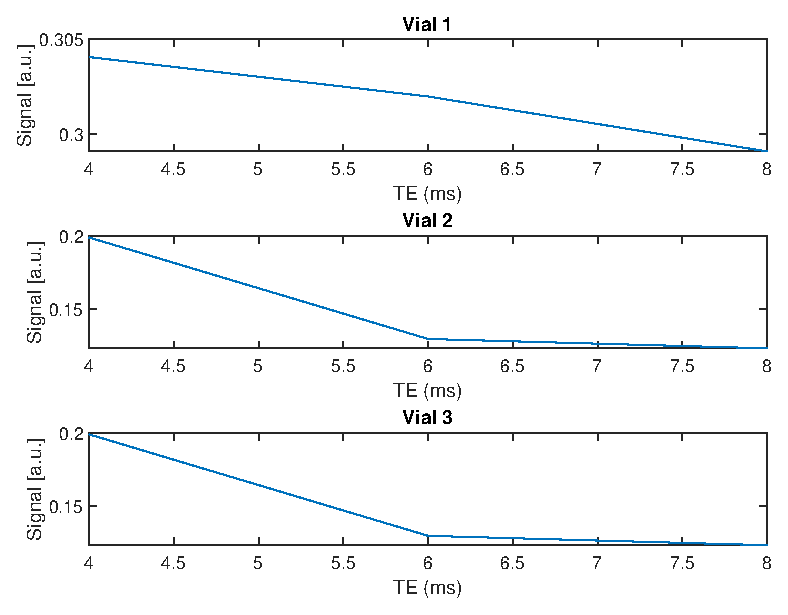
\includegraphics[width=\maxwidth{56.196688409433015em}]{figure_2}
\end{center}
\begin{matlabcode}

%Phase
figure;
subplot(3,1,1)
plot(TE,S1phase)
title('Vial 1'); xlabel 'TE (ms)'; ylabel 'Phase [rad]';
subplot(3,1,2)
plot(TE,S2phase)
title('Vial 2'); xlabel 'TE (ms)'; ylabel 'Phase [rad]';
subplot(3,1,3)
plot(TE,S3phase)
title('Vial 3'); xlabel 'TE (ms)'; ylabel 'Phase [rad]';
\end{matlabcode}
\begin{center}
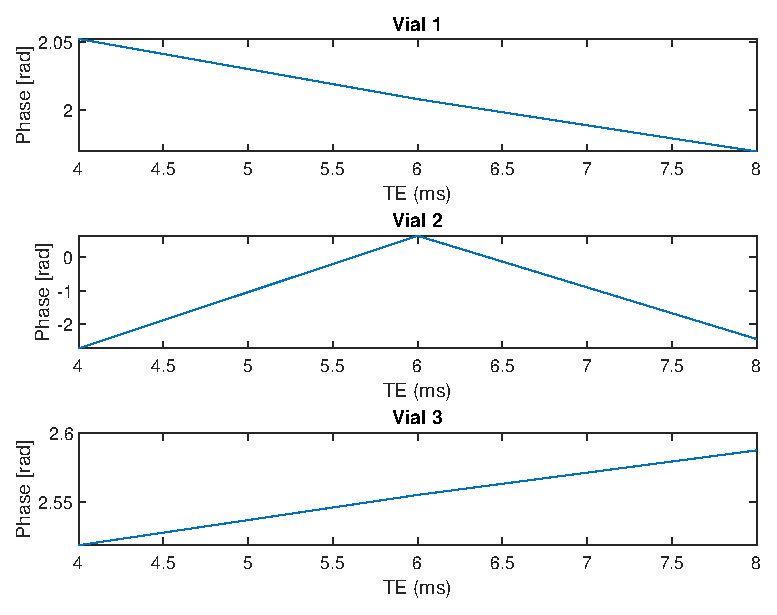
\includegraphics[width=\maxwidth{56.196688409433015em}]{figure_3}
\end{center}

\matlabheading{1d)}

\begin{par}
\begin{flushleft}
Implement a \underline{2-point Dixon} reconstruction. \textbf{Provide the water only and a fat only image of the phantom}.
\end{flushleft}
\end{par}

\vspace{1em}

\begin{par}
\begin{flushleft}
The 2-point dixon method assumes perfect field homogeneity, that fat has only 1 pure spectral component, and that the images were acquired perfectly in phase (IP) and out of phase (OP).
\end{flushleft}
\end{par}

\begin{par}
\begin{flushleft}
For the simple 2-point Dixon:
\end{flushleft}
\end{par}

\begin{par}
\begin{flushleft}
    Water = 1/2(IP + OP)
\end{flushleft}
\end{par}

\begin{par}
\begin{flushleft}
    Fat = 1/2(IP - OP)
\end{flushleft}
\end{par}

\begin{par}
\begin{flushleft}
We can further correct for the $\phi_{0\;}$ off-resonance factor by taking the absolute value of the sum of the fat and water contributions. This effectively gits rid of the initial phase offset caused by local RF penetration issues and delays in the receiver chains in the coils. This, however, still does not fix off-resonance from field homogeneity.
\end{flushleft}
\end{par}

\begin{matlabcode}
water = 0.5*abs(IP + OP);
fat = 0.5*abs(IP - OP);
figure; subplot(1,2,1); imshow(water,[]);  title('2-point Dixon - Water'); colorbar; map1b = colorbar; title(map1b,'[a.u.]');
subplot(1,2,2); imshow(fat,[]); title('2-point Dixon - Fat'); colorbar; map2b = colorbar; title(map2b,'[a.u.]');
\end{matlabcode}

\matlabheading{1e)}

\begin{par}
\begin{flushleft}
Implement a \underline{modified 2-point Dixon} reconstruction. \textbf{Provide the water only and a fat only image of the phantom.}
\end{flushleft}
\end{par}

\vspace{1em}

\begin{par}
\begin{flushleft}
In the modified Dixon method, we synthesize the third 3-point Dixon measurement from only two echoes. (At least, I assume that's what the modified 2-point Dixon method is. The lecture notes, homework instructions, or supplementary lectures slides do not explicitly describe a "modified" 2-point Dixon).
\end{flushleft}
\end{par}

\begin{par}
\begin{flushleft}
To synthesize the off-resonance factor, we can use the following formula:
\end{flushleft}
\end{par}

\begin{par}
$$2\phi^ˆ =\angle {\left(m_1^* m_2 \right)}^2$$
\end{par}

\begin{matlabcode}
phi_hat1 = 0.5*angle((conj(IP).*OP).^2);
water2 = 0.5*abs(water.*(1 + exp(1i*phi_hat1)) + fat.*(1 - exp(1i*phi_hat1)));
fat2 = 0.5*abs(water.*(1 - exp(1i*phi_hat1)) + fat.*(1 + exp(1i*phi_hat1)));
figure; subplot(1,2,1); imshow(water2,[]);  title('Modifed 2-point Dixon - Water'); colorbar; map1c = colorbar; title(map1c,'[a.u.]');
subplot(1,2,2); imshow(fat2,[]); title('Modifed 2-point Dixon - Fat'); colorbar; map2c = colorbar; title(map2c,'[a.u.]');
\end{matlabcode}
\begin{center}
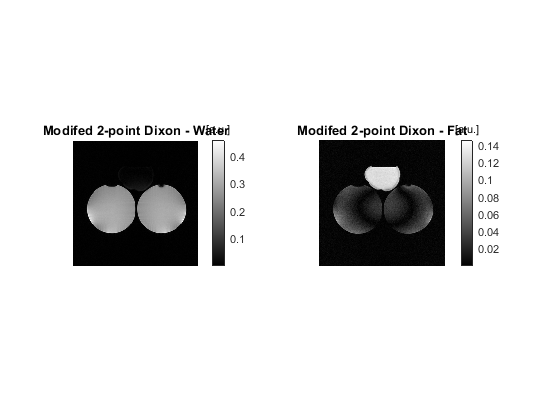
\includegraphics[width=\maxwidth{56.196688409433015em}]{figure_4}
\end{center}

\matlabheading{1f)}

\begin{par}
\begin{flushleft}
Implement a \underline{3-point Dixon} reconstruction.\textbf{ Provide the water only and a fat only image and the field map of the phantom.}
\end{flushleft}
\end{par}

\vspace{1em}

\begin{matlabcode}
phi_hat2 = 0.5*abs((angle(conj(OP).*OP_)));
water3 = 0.5*abs((IP + OP.*exp(-1i*phi_hat2)));
fat3 = 0.5*abs((IP - OP.*exp(-1i*phi_hat2)));
figure; subplot(1,2,1); imshow(water3,[]);  title('3-point Dixon - Water'); colorbar; map1 = colorbar; title(map1,'[a.u.]');
subplot(1,2,2); imshow(fat3,[]); title('3-point Dixon - Fat'); colorbar; map2 = colorbar; title(map2,'[a.u.]');
\end{matlabcode}
\begin{center}
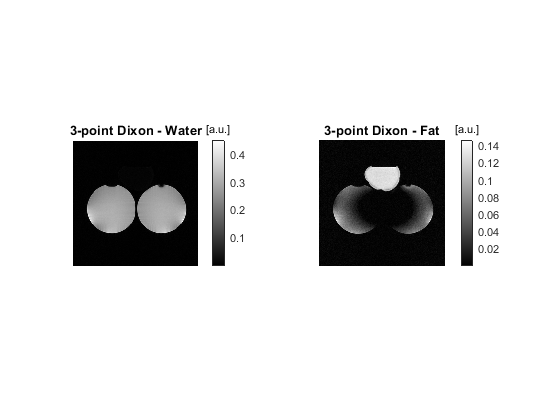
\includegraphics[width=\maxwidth{56.196688409433015em}]{figure_5}
\end{center}

\vspace{1em}

\matlabheading{1g)}

\begin{par}
\begin{flushleft}
Field Map Estimation: The phase estimate φ (in radians) can be converted to a frequency estimate (in Hz) by dividing φ by 2π ΔTE, where ΔTE is the time between the first and second images. \textbf{Generate and provide the field map.}
\end{flushleft}
\end{par}

\vspace{1em}

\begin{matlabcode}
dT = 0.002;
% Difference between IP and OP (with phase correction) yields 
field_map = (phi_hat2)/(2*pi*dT);
figure; imshow(field_map,[]); title('Field Map'); colorbar; map = colorbar; title(map,'Hz');
\end{matlabcode}
\begin{center}
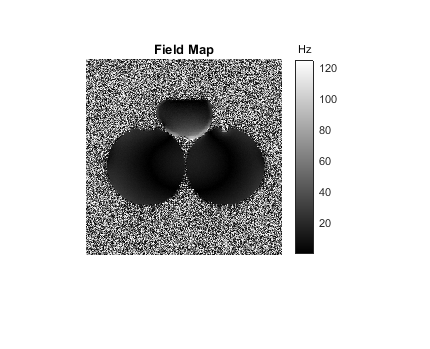
\includegraphics[width=\maxwidth{43.151028600100354em}]{figure_6}
\end{center}

\begin{par}
\begin{flushleft}
The largest susceptibility artifacts (resultant from inhomogenity) are near the bottom of the fat vial. This is most likely due to the sharp changes in material interfaces (air and water), which often result in susceptibility artifacts, such as bone-air interfaces that result in susceptibility artifact in the skull. There is also slowly varying inhomogeneity across all vials.
\end{flushleft}
\end{par}

\matlabheading{1h)}

\begin{par}
\begin{flushleft}
\textbf{Compare the results from d, e, and f.}
\end{flushleft}
\end{par}

\vspace{1em}

\begin{matlabcode}
figure; subplot(1,3,1); imshow(fat,[]); title('2-point Dixon - Fat'); colorbar; map2a = colorbar; title(map2a,'[a.u.]');
subplot(1,3,2); imshow(fat2,[]);  title('Modifed 2-point Dixon - Fat'); colorbar; map2b = colorbar; title(map1b,'[a.u.]');
\end{matlabcode}
\begin{center}
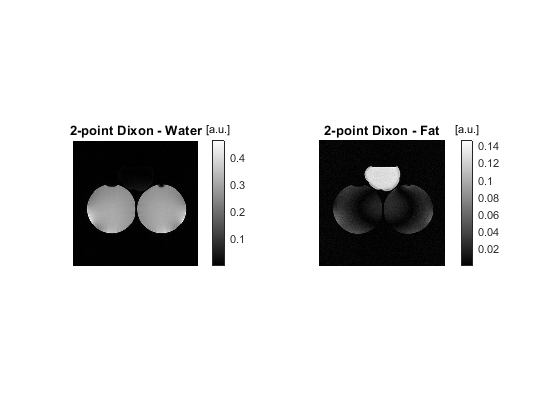
\includegraphics[width=\maxwidth{56.196688409433015em}]{figure_7}
\end{center}
\begin{matlabcode}
subplot(1,3,3); imshow(fat3,[]); title('3-point Dixon - Fat'); colorbar; map2c = colorbar; title(map2c,'[a.u.]');
\end{matlabcode}
\begin{center}
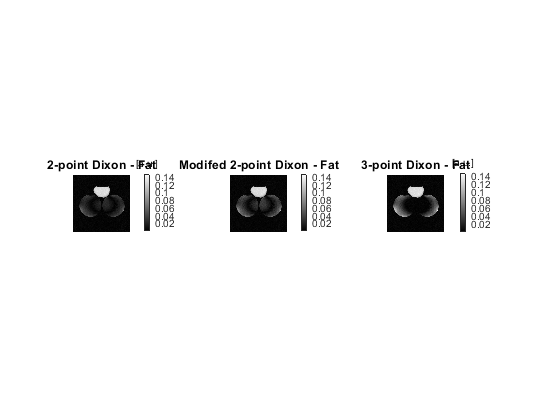
\includegraphics[width=\maxwidth{56.196688409433015em}]{figure_8}
\end{center}

\vspace{1em}

\matlabheading{\textit{Problem 2 -- In Vivo Data}}

\begin{par}
\begin{flushleft}
The in vivo data set was provided by Dr. John Pauly from Stanford University. It is saved in matlab format in the file dixon\_images.mat. There are three matlab variables, image 1, image 2, and image 3, which contain the three Dixon images. The images are from a gradient recalled sequence, with echo times of 12.8 ms, 19.2 ms, and 25.6 ms. These correspond to 2π, 3 π and 4 π phase shifts of the fat/water difference frequency, which is 72 Hz for 0.5T where these images were acquired. Before starting, take a look at the three images to get a sense of the different information they contain. The first and third have water and fat in phase, while water and fat have opposing phase in the second image. This is particularly noticeable behind the eye in the contrast between the optic nerve (water) and the retro-orbital fat.
\end{flushleft}
\end{par}

\matlabheading{1a)}

\begin{par}
\begin{flushleft}
\textbf{Run the 3 reconstructions developed in problem 1 (2-point Dixon, 2-point modified Dixon and 3-point Dixon) and compare the results.}
\end{flushleft}
\end{par}

\begin{matlabcode}
cd('../..')
load('dixon_images.mat')
img1 = image_1;
img2 = image_2;
img3 = image_3;
\end{matlabcode}

\vspace{1em}

\begin{par}
\begin{flushleft}
\underline{2-point Dixon} reconstruction.
\end{flushleft}
\end{par}

\begin{matlabcode}
Water = 0.5*abs(img2+img1);
Fat = 0.5*abs(img2-img1);
figure; subplot(1,2,1); imshow(Water,[]);  title('2-point Dixon - Water'); colorbar; map1b = colorbar; title(map1b,'[a.u.]');
subplot(1,2,2); imshow(Fat,[]); title('2-point Dixon - Fat'); colorbar; map2b = colorbar; title(map2b,'[a.u.]');
\end{matlabcode}
\begin{center}
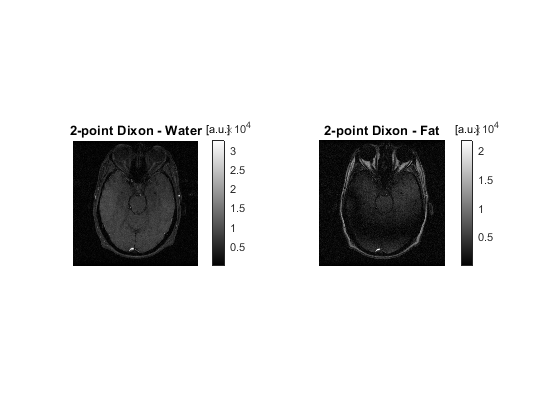
\includegraphics[width=\maxwidth{56.196688409433015em}]{figure_9}
\end{center}

\vspace{1em}

\begin{par}
\begin{flushleft}
\underline{Modified 2-point Dixon} reconstruction. 
\end{flushleft}
\end{par}

\begin{matlabcode}
Phi_hat1 = 0.5*angle((conj(img2).*img1).^2);
Water2 = 0.5*abs(Water.*(1 + exp(1i*Phi_hat1)) + Fat.*(1 - exp(1i*Phi_hat1)));
Fat2 = 0.5*abs(Water.*(1 - exp(1i*Phi_hat1)) + Fat.*(1 + exp(1i*Phi_hat1)));
figure; subplot(1,2,1); imshow(Water2,[]);  title('Modifed 2-point Dixon - Water'); colorbar; map1c = colorbar; title(map1c,'[a.u.]');
subplot(1,2,2); imshow(Fat2,[]); title('Modifed 2-point Dixon - Fat'); colorbar; map2c = colorbar; title(map2c,'[a.u.]');
\end{matlabcode}
\begin{center}
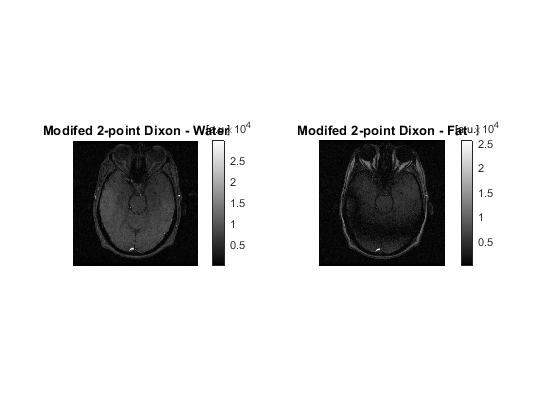
\includegraphics[width=\maxwidth{56.196688409433015em}]{figure_10}
\end{center}

\begin{par}
\begin{flushleft}
\underline{3-point Dixon} reconstruction.
\end{flushleft}
\end{par}

\begin{matlabcode}
Phi_hat2 = 0.5*abs((angle(conj(img1).*img3)));
Water3 = 0.5*abs((img2 + img1.*exp(-1i*Phi_hat2)));
Fat3 = 0.5*abs((img2 - img1.*exp(-1i*Phi_hat2)));
figure; subplot(1,2,1); imshow(Water3,[]);  title('3-point Dixon - Water'); colorbar; map1 = colorbar; title(map1,'[a.u.]');
subplot(1,2,2); imshow(Fat3,[]); title('3-point Dixon - Fat'); colorbar; map2 = colorbar; title(map2,'[a.u.]');
\end{matlabcode}
\begin{center}
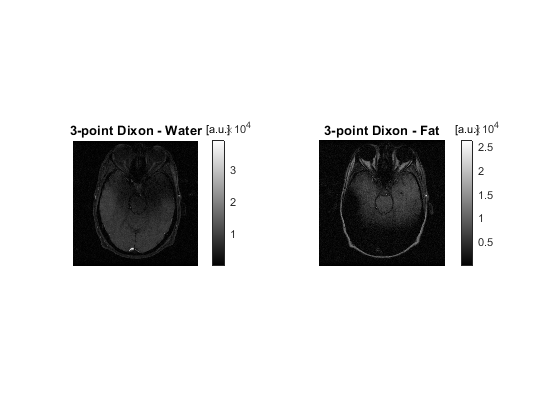
\includegraphics[width=\maxwidth{56.196688409433015em}]{figure_11}
\end{center}

\vspace{1em}

\begin{par}
\begin{flushleft}
\underline{Field Map Estimation}
\end{flushleft}
\end{par}

\begin{matlabcode}
dT = 0.002;
field_map = Phi_hat2/(2*pi*dT);
figure; imshow(field_map,[]); title('Field Map'); colorbar; map = colorbar; title(map,'Hz');
\end{matlabcode}
\begin{center}
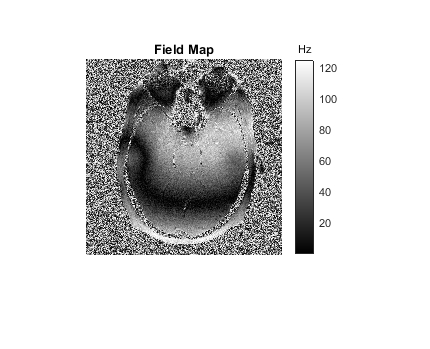
\includegraphics[width=\maxwidth{43.151028600100354em}]{figure_12}
\end{center}

\begin{center}
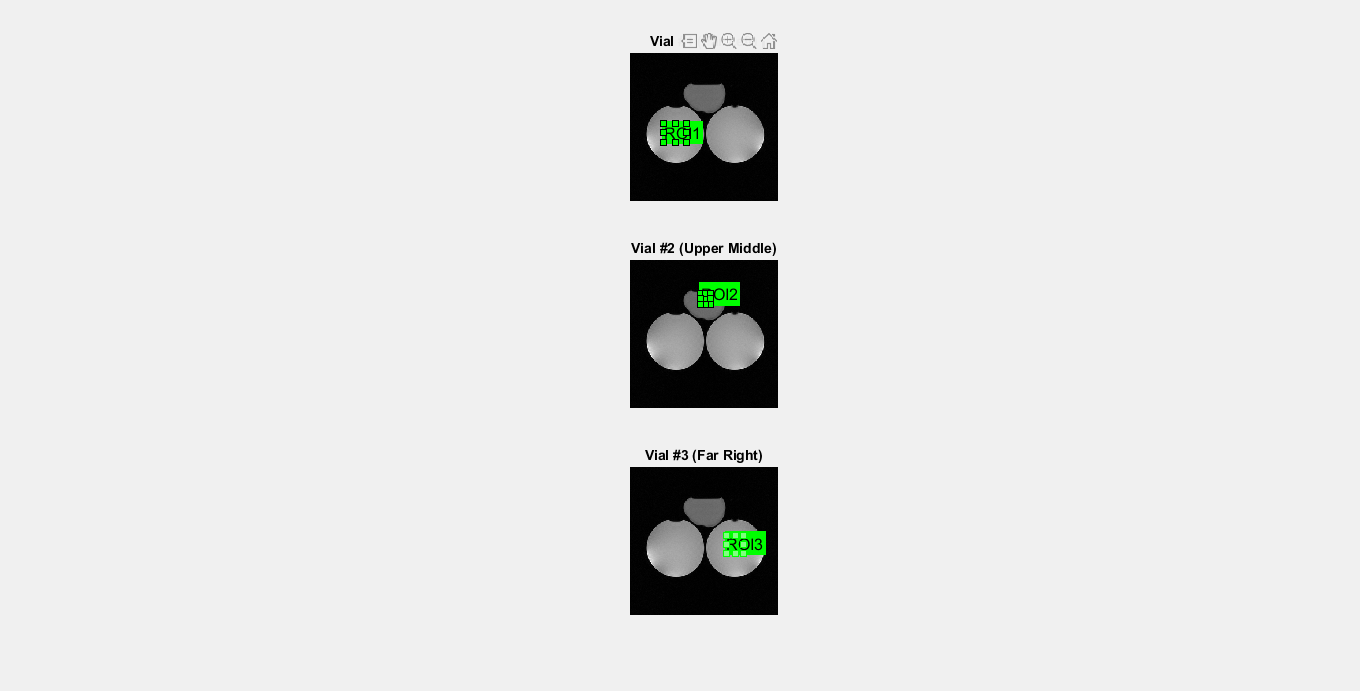
\includegraphics[width=\maxwidth{116.60812844957351em}]{figure_13}
\end{center}

\vspace{1em}

\begin{par}
\begin{flushleft}
\underline{Compare the results from d, e, and f}.
\end{flushleft}
\end{par}

\begin{matlabcode}
figure; subplot(1,3,1); imshow(Fat,[]); title('2-point Dixon - Fat'); colorbar; map2a = colorbar; title(map2a,'[a.u.]');
subplot(1,3,2); imshow(Fat2,[]);  title('Modifed 2-point Dixon - Fat'); colorbar; map2b = colorbar; title(map2b,'[a.u.]');
subplot(1,3,3); imshow(Fat3,[]); title('3-point Dixon - Fat'); colorbar; map2c = colorbar; title(map2c,'[a.u.]');
\end{matlabcode}
\begin{center}
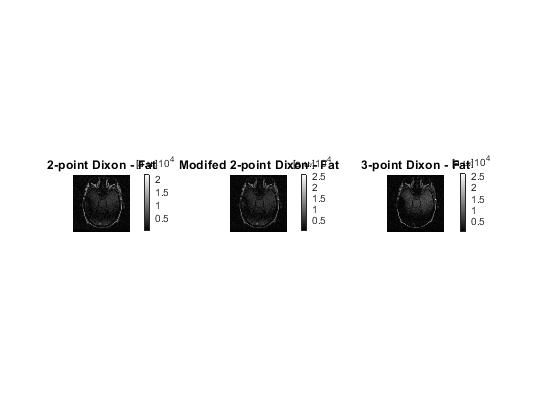
\includegraphics[width=\maxwidth{56.196688409433015em}]{figure_14}
\end{center}

\vspace{1em}


\matlabheadingtwo{Functions:}

\begin{matlabcode}
function value = lookup(fields,values,field, length)
    index = find(cellfun(@(s) strcmp(field, s), fields));
    value = cellfun(@str2num,values(index:(index+length-1)));
end
\end{matlabcode}

\end{document}
